\documentclass{article}
\usepackage{graphicx}
\usepackage{parskip}
\usepackage{float}
\usepackage{multicol}
\usepackage{hyperref}
\usepackage{makecell}
\usepackage{geometry}

\geometry{
    a4paper,
    total={160mm,240mm},
    left=20mm,
    top=20mm,
}

\begin{document}

\begin{center}
    \begin{figure}
        \centering
        
\includegraphics[width = 4cm]{Logo.png}
    \end{figure}
    \par
    02312, 62531, 02314 og 62532.
    \par
    \underline{Development Methods for IT Systems Fall 23}
\end{center}

\hrulefill

\begin{center}
    \LARGE{CDIO 3 Report} \\
    \Large{Group 3}
\end{center}

\hrulefill

\par

\begin{figure} [H]
    
\includegraphics[width=.20\textwidth]{Samin.png}\hfill
    
\includegraphics[width=.20\textwidth]{Daniall.png}\hfill
    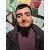
\includegraphics[width=.20\textwidth]{Andrei.png}\hfill
    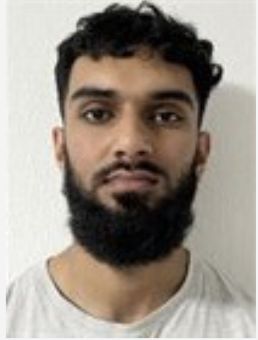
\includegraphics[width=.20\textwidth]{Abdullah.png}
\end{figure}
\begin{multicols}{4}
Chowdhury, \\
Samin \\
S235078
\vfill\null
\columnbreak
Mudasar, \\
Daniall \\
S235070
\vfill\null
\columnbreak
Enache, \\
Andrei \\
S235089
\vfill\null
\columnbreak
Hassan, \\
Abdullah \\
S235769
\vfill\null
\end{multicols}

\begin{center}
    \Large{Software Technology and IT Electronics} \\
    \Large{27-10-2023}
\end{center}

\pagebreak

\section{Summary}
\section{Hourly Accounting}
\begin{center}
    \begin{tabular}{| c | c | c | c |}
      \hline
      30th of October & \makecell{Daniall, Andrei \\ Abdullah} & \underline{1 hour} & \makecell{Discussed general \\ structure of the program, and \\ distributed duties, \\ created doc and repository} \\
      \hline
      1st of November & \makecell{Daniall, Andrei \\ Abdullah} & \underline{4 hours} & \makecell{Discussed basic \\ programming principles \\ and created the report} \\
      \hline
    \end{tabular}
\end{center}

\pagebreak

\tableofcontents

\pagebreak

\section{Introduction}
Lorem ipsum dolor sit amet, consectetur adipiscing elit. Morbi at sem condimentum, vestibulum dui sit
amet, ultricies mi. Phasellus commodo ut est tincidunt dictum. Pellentesque non leo arcu. Nullam nec
eleifend diam, non ultricies eros. Etiam posuere, arcu vel volutpat bibendum, nunc mi sollicitudin erat,
mattis faucibus ipsum nisi ut mauris. In in pretium lectus, id feugiat dolor. Suspendisse id dui placerat,
sodales est vitae, luctus arcu. In nec porttitor velit. Vivamus eget sollicitudin nulla. Curabitur sodales
sagittis arcu.
\par
Nunc varius elit ac sagittis commodo. Nulla facilisi. Donec at lacus dictum felis tempus fermentum eu
non felis. Sed molestie, justo eu aliquam porta, elit odio facilisis leo, molestie ullamcorper velit mauris
quis diam. Proin tempus sagittis vestibulum. Curabitur molestie tortor eu ornare viverra. Donec risus
ligula, tristique vel ligula vitae, blandit faucibus leo. Cras at mauris massa.
\section{Project Planning}
\section{Requirements/Analysis}
\subsection{Vision of the Customer}
\subsection{Requirements List}
\subsection{Use Case Diagram}
\subsection{Domain Model}
\subsection{System Sequence Diagram}
\section{Design}
\subsection{Class Diagram}
\subsection{Sequence Diagram}
\section{Implementation}
\section{Testing}
\section{Configuration}
\subsection{Minimum Requirements}
\subsection{Installation and Running Instructions}
\section{Conclusion}
\section{Appendix}
\subsection{Literature}
\subsection{Code}
\subsection{Figures}

\end{document}
